% IS-RAG — preprint arXiv, versão pt-BR (sem ACL .sty)
% Compilar com: pdflatex main-ptbr.tex  (duas vezes, depois bibtex, duas vezes)
% Requer apenas pacotes padrão do TeX Live.
\documentclass[11pt,a4paper]{article}

% --- Layout ---
\usepackage[margin=2.5cm]{geometry}
\usepackage{multicol}
\usepackage{titlesec}
\usepackage{parskip}

% --- Fonte & Codificação ---
\usepackage[T1]{fontenc}
\usepackage[utf8]{inputenc}
\usepackage[brazilian]{babel}
\usepackage{times}
\usepackage{microtype}

% --- Matemática ---
\usepackage{amsmath,amssymb}

% --- Tabelas & Figuras ---
\usepackage{booktabs}
\usepackage{graphicx}
\usepackage{multirow}
\usepackage{array}
\usepackage{caption}
\usepackage{float}

% --- Listas ---
\usepackage{enumitem}

% --- Cor ---
\usepackage{xcolor}

% --- Algoritmos ---
\usepackage{algorithm}
\usepackage{algpseudocode}
\renewcommand{\algorithmicrequire}{\textbf{Entrada:}}
\renewcommand{\algorithmicensure}{\textbf{Saída:}}

% --- Listagens de código ---
\usepackage{listings}
\lstset{
  basicstyle=\ttfamily\small,
  breaklines=true,
  frame=single,
  backgroundcolor=\color{gray!8},
  columns=fullflexible,
  keepspaces=true,
  literate={á}{{\'a}}1 {ã}{{\~a}}1 {â}{{\^a}}1 {à}{{\`a}}1
           {é}{{\'e}}1 {ê}{{\^e}}1
           {í}{{\'i}}1
           {ó}{{\'o}}1 {ô}{{\^o}}1 {õ}{{\~o}}1
           {ú}{{\'u}}1 {ü}{{\"u}}1
           {ç}{{\c{c}}}1
           {Á}{{\'A}}1 {Ã}{{\~A}}1 {É}{{\'E}}1 {Ó}{{\'O}}1 {Ú}{{\'U}}1
}

% --- Hiperlinks ---
\usepackage[colorlinks=true,linkcolor=blue!70!black,citecolor=blue!70!black,urlcolor=blue!70!black]{hyperref}

% --- Bibliografia ---
\usepackage[round,sort,authoryear]{natbib}
\bibliographystyle{plainnat}

% --- Formatação de seções (estilo ACL) ---
\titleformat{\section}{\normalsize\bfseries}{\thesection.}{0.5em}{}
\titleformat{\subsection}{\normalsize\itshape}{\thesubsection.}{0.5em}{}
\titleformat{\paragraph}[runin]{\normalsize\bfseries}{}{0pt}{}[~~]
\titlespacing{\section}{0pt}{6pt}{3pt}
\titlespacing{\subsection}{0pt}{4pt}{2pt}

% --- Placeholder de figura ---
\newcommand{\figplaceholder}[2]{%
  \begin{center}
    \fbox{\parbox[c][#1][c]{0.92\linewidth}{%
      \centering\color{gray}\small [Figura — #2]%
    }}
  \end{center}%
}

% --- Ambiente de resumo ---
\renewenvironment{abstract}{%
  \small\begin{center}{\bfseries Resumo}\end{center}%
  \begin{quote}\small
}{%
  \end{quote}\bigskip
}

% =================================================================
\begin{document}

% --- Bloco de título ---
\begin{center}
  {\Large\bfseries IS-RAG: Geração Aumentada por Recuperação\\
   baseada em Esquemas Imagéticos para Busca Cognitiva\\
   em Discurso Político}

  \vspace{0.8em}

  {\normalsize
    Yan Justino$^{1,2}$ \\[4pt]
    $^1$ CESAR School \quad $^2$ Itaú Unibanco \\[4pt]
    \texttt{contact@yanjustino.com}
  }

  \vspace{0.6em}
  \rule{\linewidth}{0.4pt}
\end{center}

% =================================================================
\begin{abstract}
\textbf{Objetivo.}
Sistemas de recuperação densa falham quando o usuário e o documento
expressam a mesma estrutura conceitual por vocabulários distintos —
fenômeno que denominamos \emph{lacuna léxico-cognitiva}.
Este artigo apresenta o \textbf{IS-RAG}, um estudo piloto que investiga
se a indexação explícita de \emph{esquemas imagéticos}
\citep{lakoff1980,talmy1988} — padrões pré-linguísticos como
\textsc{Force}, \textsc{Container} e \textsc{Path} — pode superar essa
lacuna em um corpus de discurso político em português.

\textbf{Método.}
Durante a indexação, um \emph{Analisador Cognitivo} baseado em LLM
anota cada trecho com os esquemas imagéticos presentes, gerando
metadados estruturados armazenados juntamente com dois embeddings
vetoriais independentes: um textual e um cognitivo (768d cada).
Em tempo de consulta, os esquemas detectados na consulta disparam um
\emph{boost proporcional} sobre os trechos que compartilham a mesma
estrutura cognitiva, possibilitando recuperação orientada por metáfora
abstrata além da sobreposição lexical.

\textbf{Avaliação.}
Construímos um ground truth estilo TREC sobre 121 discursos
parlamentares brasileiros (171 trechos), com 10 consultas válidas
(3~\textsc{Force} $+$ 3~\textsc{Container} $+$ 3~\textsc{Path} $+$
1~cross-schema) anotadas por LLM independente (\texttt{claude-opus-4-7},
distinto do Analisador Cognitivo) em escala 0--3.
A métrica principal é NDCG@5; a linha de base é recuperação densa sem
boosting cognitivo.

\textbf{Achados.}
Uma ablação sobre três modos de recuperação revela que o
\emph{boosting no modo texto} — boost cognitivo proporcional aplicado
sobre similaridade textual — é a configuração mais eficaz, atingindo
NDCG@5 médio de 0,7793 contra 0,6881 da linha de base
($\Delta = +0{,}091$).
Usar o embedding cognitivo como vetor de busca primário degrada o
desempenho ($\Delta_\text{cognitivo} = -0{,}192$;
$\Delta_\text{híbrido} = -0{,}090$), localizando a contribuição do
IS-RAG no mecanismo de boosting, e não na recuperação dual.
Consultas \textsc{Force} beneficiam-se de forma mais consistente
($\Delta_\text{FORCE} = +0{,}267$); \textsc{Path} é positivo em todas
as três consultas ($\Delta_\text{PATH} = +0{,}085$);
\textsc{Container} apresenta efeito médio próximo de zero
($\Delta_\text{CONT} = -0{,}017$).
Dois achados metodológicos adicionais emergem: (1)~consultas devem ser
formuladas como \emph{afirmações metafóricas assertivas} para ativar o
componente cognitivo; (2)~frequência de esquema no corpus não prediz
\emph{boostabilidade} — esquemas convencionalizados não carregam sinal
discriminativo de re-ranking.
\end{abstract}

\noindent\textbf{Palavras-chave:} geração aumentada por recuperação $\cdot$ esquemas imagéticos $\cdot$ linguística cognitiva $\cdot$ recuperação de informação $\cdot$ processamento de linguagem natural $\cdot$ detecção de metáfora $\cdot$ recuperação densa $\cdot$ discurso político $\cdot$ busca semântica $\cdot$ cognição corporificada

% =================================================================
\section{Introdução}
\label{sec:intro}

A Geração Aumentada por Recuperação \citep{lewis2020rag} tipicamente
fundamenta a recuperação de documentos em similaridade lexical superficial
ou semântica densa.
Isso funciona bem quando o vocabulário da consulta se sobrepõe ao
vocabulário do documento, mas falha diante de uma \emph{lacuna
léxico-cognitiva}: o usuário e o documento expressam a mesma estrutura
conceitual usando palavras diferentes, frequentemente porque ambos se
apoiam em metáforas corporais subjacentes que mapeiam a experiência
espacial física sobre domínios abstratos \citep{johnson1987,lakoff1980}.

Considere uma consulta sobre \emph{pressão econômica sobre as famílias}
e um discurso parlamentar sobre \emph{instituições que se bloqueiam
mutuamente em uma disputa constitucional}.
Ambos invocam o esquema imagético \textsc{Force}/\textsc{Compulsion} —
um agente externo exercendo força sobre um paciente —, porém seus
vocabulários compartilham pouca sobreposição, tornando a recuperação densa
padrão incapaz de superar essa lacuna.

\emph{Esquemas imagéticos} \citep{johnson1987,feldman2006} são padrões
pré-linguísticos e corporificados (\textsc{Container}, \textsc{Path},
\textsc{Force}) que recorrem como metáforas estruturais em todos os
domínios do raciocínio abstrato.
Nossa hipótese é que indexar esses esquemas explicitamente e combiná-los
em tempo de consulta viabiliza uma forma de recuperação estrutural
profunda que complementa a busca semântica densa.

\paragraph{Contribuições.}
\begin{itemize}[noitemsep,topsep=2pt]
  \item Apresentamos o IS-RAG, uma técnica que indexa metadados de
        esquemas imagéticos juntamente com embeddings vetoriais duais
        (texto e cognitivo) e aplica boosting cognitivo proporcional
        em tempo de recuperação (\S\ref{sec:method}).
  \item Construímos um ground truth estilo TREC sobre um corpus real de
        discursos parlamentares brasileiros (171 trechos, 10 consultas
        válidas, LLM como anotador) e reportamos NDCG@5 (\S\ref{sec:eval}).
  \item Identificamos restrições metodológicas para avaliação de
        recuperação ciente de esquemas: formulação assertiva de consultas,
        frequência vs.\ boostabilidade de esquemas e risco de circularidade
        com LLM (\S\ref{sec:discussion}).
\end{itemize}

% =================================================================
\section{Trabalhos Relacionados}
\label{sec:related}

\paragraph{Geração Aumentada por Recuperação.}
\citet{lewis2020rag} introduziram o RAG para fundamentar a geração em
passagens recuperadas.
A recuperação densa com representações bi-encoder
\citep{karpukhin2020dpr} tornou-se o backbone padrão.
Extensões exploram busca híbrida esparsa-densa, re-ranking e augmentação
por conhecimento estruturado, mas nenhuma incorpora metáfora espacial
pré-linguística como sinal de recuperação.

\paragraph{Metáfora em PLN.}
A detecção automática de metáfora foi estudada como classificação ou
extração de spans \citep{shutova2010,tsvetkov2014}.
\citet{wachowiak2023,wachowiak-gromann-2022-systematic} exploram LLMs
para identificação de metáforas.
Esses trabalhos focam na \emph{detecção} de metáforas; o IS-RAG é o
primeiro, ao nosso conhecimento, a utilizar a estrutura de esquema
imagético detectado como \emph{sinal de pontuação de recuperação}.

\paragraph{Linguística Cognitiva e RI.}
Esquemas imagéticos como universais cognitivos foram formalizados por
\citet{lakoff1980}, \citet{johnson1987} e \citet{talmy1988}.
\citet{feldman2006} discute sua base neural.
Nenhum trabalho anterior em Recuperação de Informação indexa documentos
por esquema imagético e utiliza correspondência de esquemas para boosting
de recuperação.

\paragraph{PLN em Português e corpora parlamentares.}
Modelos de linguagem pré-treinados para o português brasileiro
\citep{souza2020bertimbau} demonstraram que o pré-treinamento
específico ao idioma melhora substancialmente o desempenho em tarefas
downstream em relação a modelos multilíngues genéricos.
O discurso parlamentar em português foi estudado por meio do
Corpus Ulysses \citep{albuquerque2022ulyssesner}, coleção de documentos
legislativos da Câmara dos Deputados brasileira utilizada para
classificação de textos, reconhecimento de entidades e análise semântica.
Nosso corpus de avaliação é extraído da mesma fonte institucional via
mesma API aberta e estende os recursos existentes com anotações de
esquemas imagéticos e julgamentos de relevância graduada para avaliação
de recuperação.
Análises de enquadramento e sentimento em texto político brasileiro
\citep{vargas2021bert} fornecem precedente adicional para abordagens
computacionais da estrutura ideológica na linguagem parlamentar em
português.

% =================================================================
\section{Método}
\label{sec:method}

A Figura~\ref{fig:pipeline} ilustra o pipeline IS-RAG.
O pseudocódigo formal encontra-se no Apêndice~\ref{app:algorithms}.

\begin{figure}[H]
  \centering
  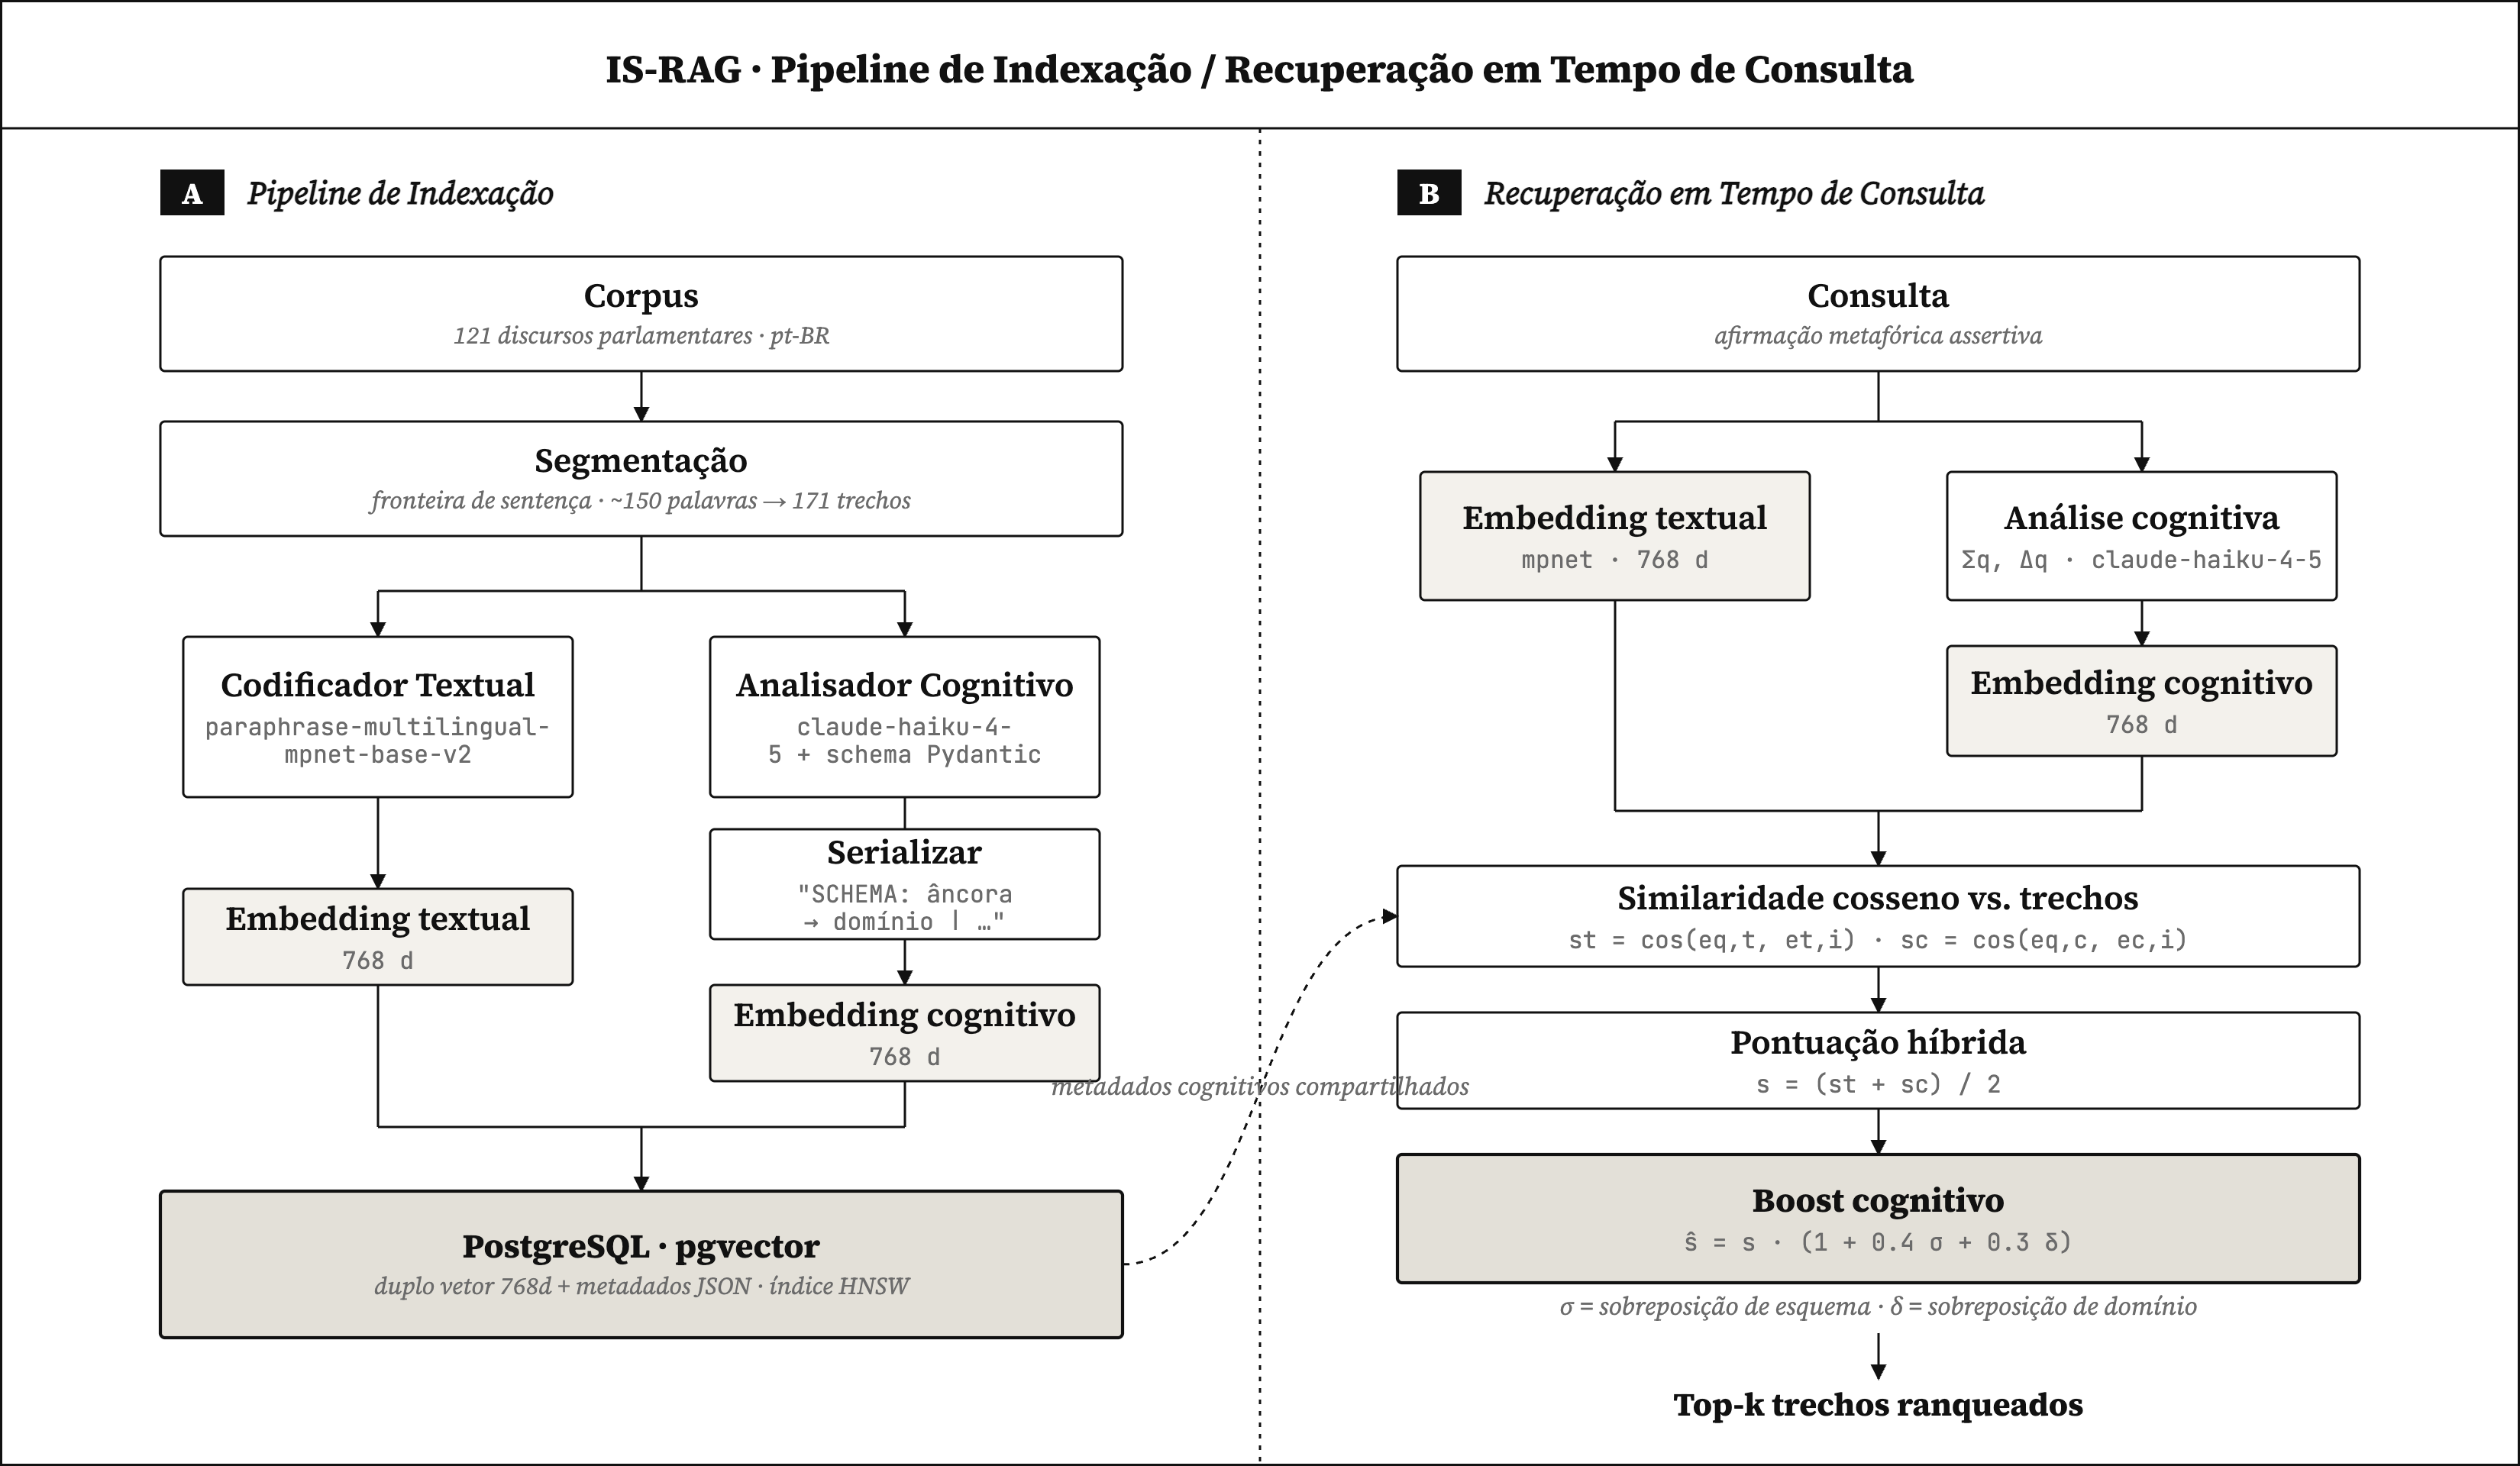
\includegraphics[width=1\textwidth]{images/PT_Pipeline_pt-br_.png}
  \caption{Visão geral do IS-RAG: etapas de indexação e recuperação.}
  \label{fig:pipeline}
\end{figure}

\subsection{Corpus e Segmentação}

O corpus compreende 121 discursos parlamentares brasileiros em
\textbf{português}, coletados da API aberta da Câmara dos Deputados
(\url{dados.camara.leg.br/api/v2}), abrangendo janeiro a dezembro
de~2025.
Os discursos são estratificados por espectro ideológico (esquerda,
centro, direita) em 13 partidos.
Cada discurso é segmentado em trechos de aproximadamente 150~palavras
por meio de divisão em fronteiras de sentenças, gerando 171~trechos
(média de 2,7 por discurso).

\subsection{Embeddings Duais}

Cada trecho produz dois vetores independentes de 768 dimensões:

\begin{enumerate}[noitemsep,topsep=2pt]
  \item \textbf{Embedding textual:} representação densa do texto bruto
        do trecho via \textit{paraphrase-multilingual-mpnet-base-v2}
        \citep{reimers2019sbert}, executado localmente em CPU.
  \item \textbf{Embedding cognitivo:} representação densa dos metadados
        cognitivos serializados no formato
        \texttt{"SCHEMA: âncora $\to$ domínio $|$ \ldots"}, capturando
        a estrutura esquemático-imagética independentemente do vocabulário
        literal.
\end{enumerate}

Ambos os vetores são armazenados no PostgreSQL~16 com a extensão
\texttt{pgvector} e indexados via HNSW para busca aproximada do
vizinho mais próximo.

Escolhemos deliberadamente o \texttt{paraphrase-multilingual-mpnet-base-v2}
em vez de APIs comerciais de embedding mais recentes por duas razões.
Primeiro, \emph{reprodutibilidade}: todos os embeddings são gerados
localmente, sem acesso a API, limites de taxa ou custos de uso,
possibilitando replicação integral do experimento.
Segundo, \emph{adequação}: o modelo oferece cobertura validada do
português em um espaço de 768 dimensões suficiente para a escala de
prova de conceito deste trabalho (171~trechos), e seu treinamento
multilíngue inclui o português brasileiro \citep{souza2020bertimbau}.
Não afirmamos que a substituição por modelos de embedding maiores ou
mais recentes não melhoraria os resultados; isso é um item explícito da
agenda futura (\S\ref{sec:conclusion}), mas é ortogonal à variável sob
investigação — o próprio sinal de boosting cognitivo.

\subsection{Analisador Cognitivo}

O Analisador Cognitivo envia cada trecho para o
\texttt{claude-haiku-4-5} \citep{anthropic2024} usando um prompt
compartilhado (disponível em \url{https://github.com/yanjustino/is-rag}) e extrai JSON estruturado
validado por um schema Pydantic.
A taxonomia segue \citet{lakoff1980} e \citet{talmy1988}:

\begin{center}
\small
\begin{tabular}{ll}
\toprule
\textbf{Esquema} & \textbf{Subtipos} \\
\midrule
\textsc{Container} & Inside, Outside, Boundary, Intrusion \\
\textsc{Path}      & Source, Trajectory, Goal, Diversion \\
\textsc{Force}     & Blockage, Compulsion, Resistance, Counter\_Force \\
\bottomrule
\end{tabular}
\end{center}

Uma \emph{regra de literalidade} instrui o modelo a retornar listas
vazias para textos não-metafóricos, prevenindo esquemas alucinados.
Os trechos são processados concorrentemente (5 workers) para reduzir
o tempo de ingestão.
O corpus apresenta 92~ocorrências de \textsc{Path}, 88~de
\textsc{Container} e 83~de \textsc{Force} nos 171~trechos.

\subsection{Busca Híbrida e Boosting Cognitivo}
\label{sec:boosting}

O IS-RAG suporta três modos de recuperação.
Em todos os três, o Analisador Cognitivo executa sobre a consulta em
tempo de recuperação para detectar esquemas ($\Sigma_q$) e domínios
alvo ($\Delta_q$).
Os modos diferem apenas na forma como a similaridade base~$s$ é
computada antes do boost:

\begin{itemize}[noitemsep,topsep=2pt]
  \item \textbf{Texto:} $s = \cos(\mathbf{e}_{q,t},\,\mathbf{e}_{t,i})$
        — o embedding textual da consulta é comparado contra os
        embeddings textuais dos trechos.
        A informação cognitiva contribui apenas via boost.
  \item \textbf{Cognitivo:} $s = \cos(\mathbf{e}_{q,c},\,\mathbf{e}_{c,i})$
        — a saída do Analisador Cognitivo para a consulta é serializada
        no mesmo formato \texttt{schema\,$\to$\,domínio} da indexação,
        embutida e comparada contra os embeddings cognitivos dos trechos.
  \item \textbf{Híbrido:} $s = \bigl(s_t + s_c\bigr)/2$
        — média aritmética das similaridades textual e cognitiva.
\end{itemize}

Após computar~$s$, o mesmo \emph{boost cognitivo proporcional} é
aplicado nos três modos:

\begin{equation}
  \label{eq:boosting}
  \hat{s} = s \cdot \bigl(1 + 0{,}4\,\sigma + 0{,}3\,\delta\bigr)
\end{equation}

\noindent onde $\sigma$ é a fração dos detalhes cognitivos de um trecho
cujo \texttt{schema\_name} corresponde a um esquema em~$\Sigma_q$,
e $\delta$ é a fração análoga para \texttt{target\_domain}
em relação a~$\Delta_q$.
Os pesos ($\alpha{=}0{,}4$, $\beta{=}0{,}3$) foram definidos por
design; a estrutura esquemática é o sinal primário e o domínio é o
reforço secundário.
A linha de base desativa o Analisador Cognitivo inteiramente e aplica
recuperação puramente por embedding textual sem boosting.

% =================================================================
\section{Configuração da Avaliação}
\label{sec:eval}

\paragraph{Construção do Ground Truth.}
Construímos um ground truth por pooling estilo TREC \citep{voorhees2005}.
Para cada consulta, o IS-RAG (híbrido) e a linha de base recuperam
independentemente os 10 trechos mais relevantes; a união
($\approx$14--18 trechos únicos por consulta) é anotada quanto à
relevância (0--3) por um LLM (\texttt{claude-opus-4-7}).
Pontuações~$\geq 2$ exigem que o anotador cite uma palavra-âncora e
o subtipo de esquema como evidência rastreável.
Consultas com IDCG$=0$ (nenhum trecho com pontuação~$\geq 2$) são
excluídas \citep{buckley2004}.

\paragraph{Projeto das Consultas.}
Dez consultas válidas foram projetadas com três propriedades:
(1)~cobertura taxonômica (3~\textsc{Force} $+$ 3~\textsc{Container}
$+$ 3~\textsc{Path} $+$ 1~cross-schema);
(2)~lacuna lexical deliberada (as consultas usam linguagem metafórica
assertiva, evitando o vocabulário literal esperado nos documentos);
(3)~cenários entre domínios (as consultas visam esquemas que aparecem
em domínios distintos do domínio da própria consulta).

\paragraph{Métrica.}
Reportamos NDCG@5 \citep{jarvelin2002}.
O MRR foi rejeitado: com múltiplos documentos relevantes em diferentes
graus de relevância, o MRR satura em~1,0 independentemente da qualidade
do ranqueamento \citep{buckley2004}.

% =================================================================
\section{Resultados}
\label{sec:results}

\subsection{Ablação por Modo de Recuperação}
\label{sec:ablation}

A Tabela~\ref{tab:modes} compara os três modos de recuperação IS-RAG
contra a linha de base.
O modo texto é a única configuração que supera a linha de base;
os modos cognitivo e híbrido degradam a recuperação.

\begin{table}[H]
\centering
\small
\setlength{\tabcolsep}{6pt}
\begin{tabular}{lccc}
\toprule
\textbf{Modo} & \textbf{IS-RAG} & \textbf{Base} & $\boldsymbol{\Delta}$ \\
\midrule
\textbf{Texto}   & \textbf{0,7793} & 0,6881 & \textbf{+0,091} \\
Híbrido          & 0,5979          & 0,6881 & $-$0,090 \\
Cognitivo        & 0,4958          & 0,6881 & $-$0,192 \\
\midrule
Linha de base    & —               & 0,6881 & — \\
\bottomrule
\end{tabular}
\caption{NDCG@5 médio nas 10~consultas por modo de recuperação
  (anotador Opus independente).
  O modo texto é a configuração IS-RAG mais eficaz.}
\label{tab:modes}
\end{table}

A Tabela~\ref{tab:modes_compare} detalha $\Delta$ NDCG@5 por consulta
nos três modos, revelando quais consultas e famílias de esquema
impulsionam os resultados agregados.

\begin{table}[H]
\centering
\small
\setlength{\tabcolsep}{4pt}
\begin{tabular}{clccc}
\toprule
\textbf{Q} & \textbf{Esquema / Domínio} & \textbf{$\Delta$ Texto} & \textbf{$\Delta$ Cog.} & \textbf{$\Delta$ Híb.} \\
\midrule
Q1  & \textsc{Cont.}/Inside / Saúde             & 0,000           & $-$0,396        & $-$0,362 \\
Q2  & \textsc{Force}/Compulsion / Economia     & \textbf{+0,390} & +0,138          & +0,138 \\
Q3  & \textsc{Force}/Counter\_F / Justiça      & \textbf{+0,221} & $-$0,504        & $-$0,277 \\
Q4  & \textsc{Force}/Resistance / Política     & \textbf{+0,189} & +0,236          & +0,150 \\
\midrule
Q5  & \textsc{Cont.}/Intrusion / Justiça       & $-$0,096        & $-$0,221        & $-$0,191 \\
Q6  & \textsc{Cont.}/Outside / Dir.\ Hum.      & +0,046          & $-$0,172        & +0,046 \\
\midrule
Q7  & \textsc{Path}/Trajectory / Economia      & +0,036          & $-$0,188        & $-$0,007 \\
Q8  & \textsc{Path}/Source / Política          & \textbf{+0,111} & $-$0,555        & $-$0,424 \\
Q9  & \textsc{Path}/Diversion / Política       & +0,109          & $-$0,225        & +0,120 \\
\midrule
Q10 & \textsc{Force+Path} / Rel.\ Int.          & $-$0,094        & $-$0,038        & $-$0,094 \\
\midrule
\multicolumn{2}{l}{\textbf{Média}} & \textbf{+0,091} & $-$0,192 & $-$0,090 \\
\bottomrule
\end{tabular}
\caption{$\Delta$ NDCG@5 por consulta nos três modos IS-RAG
  (anotador Opus independente, 10~consultas).
  Q1 (\textsc{Container}/\textsc{Inside}) exibe $\Delta{=}0$ no modo
  texto: o boost é inerte para o subtipo mais convencionalizado.
  O modo texto é o mais consistentemente positivo.}
\label{tab:modes_compare}
\end{table}

\paragraph{Por que o modo cognitivo falha.}
No modo cognitivo, strings de esquema serializadas são os únicos
vetores de busca.
Com 171~trechos compartilhando esquemas sobrepostos
(PATH~92$\times$, CONTAINER~88$\times$, FORCE~83$\times$), as
similaridades de cosseno ficam comprimidas, produzindo um ranqueamento
base ruidoso que o boosting não consegue corrigir
($\Delta = -0{,}192$).

\paragraph{Por que o modo híbrido falha.}
O modo híbrido calcula a média de $s_t$ e $s_c$ antes do boosting.
O componente ruidoso do embedding cognitivo contamina o sinal textual,
rebaixando o ranqueamento base abaixo do que a recuperação textual pura
alcança ($\Delta = -0{,}090$).

\paragraph{Implicação arquitetural.}
O valor do IS-RAG reside em um \emph{sinal proporcional de
re-ranqueamento} derivado dos metadados de esquema ($\sigma$,~$\delta$),
não na recuperação por embedding duplo.
A coluna \texttt{cognitive\_embedding} é necessária para indexação
(para calcular $\sigma$), mas contraproducente como vetor de busca.
Manter \texttt{cognitive\_metadata} e usar apenas a similaridade textual
como base captura o ganho integral do IS-RAG sem a degradação dos modos
híbrido e cognitivo.

\subsection{Validação de Robustez: Efeito de Eco do LLM}
\label{sec:robustness}

Para descartar o eco do LLM como fonte do ganho no modo texto,
re-anotamos o pool de relevância com \texttt{claude-opus-4-7}, modelo
independente do \texttt{claude-haiku-4-5} usado como Analisador Cognitivo
na indexação.
A Tabela~\ref{tab:annotator} reporta o NDCG@5 no modo texto sob ambos
os anotadores.
O $\Delta$ mantém-se dentro de um ponto percentual ($+0{,}091$
vs.\ $+0{,}093$); o anotador independente também resolve uma consulta
anteriormente inanotável (Q1 \textsc{Container}/\textsc{Inside},
IDCG${=}0$ com Haiku), expandindo a avaliação para 10~consultas válidas.

\begin{table}[H]
\centering
\small
\setlength{\tabcolsep}{5pt}
\begin{tabular}{llcccc}
\toprule
\textbf{Anotador} & \textbf{Relação com parser} & \textbf{Consultas} & \textbf{Base} & \textbf{IS-RAG} & \textbf{$\Delta$} \\
\midrule
\texttt{claude-haiku-4-5} & Mesmo modelo &  9 & 0,6947 & 0,7873 & \textbf{+0,093} \\
\texttt{claude-opus-4-7}  & Independente & 10 & 0,6881 & 0,7793 & \textbf{+0,091} \\
\bottomrule
\end{tabular}
\caption{NDCG@5 (modo texto) sob dois anotadores.
  O ganho persiste ($\Delta \approx +0{,}09$) com avaliador
  independente, descartando eco do LLM como explicação principal.}
\label{tab:annotator}
\end{table}

\subsection{Fronteira de Utilidade do Embedding}
\label{sec:embedding}

Para testar se o ganho no modo texto sobrevive a um embedding base mais
forte, re-indexamos o corpus com \texttt{BAAI/bge-m3} (1024d) e
re-anotamos o pool com o mesmo anotador Opus independente.
A Tabela~\ref{tab:embedding} compara o $\Delta$ IS-RAG nos três modos
para ambos os modelos.
O ganho no modo texto colapsa para $\Delta \approx 0$; a degradação dos
modos híbrido e cognitivo permanece estável entre os modelos.
Q4 (\textsc{Force}/\textsc{Resistance}) é o principal fator do colapso:
sua baseline sobe de $0{,}489$ (mpnet) para $0{,}830$ (bge-m3),
indicando que o modelo mais forte recupera os documentos corretos sem
auxílio de esquemas.

\begin{table}[H]
\centering
\small
\setlength{\tabcolsep}{4pt}
\begin{tabular}{lccc}
\toprule
\textbf{Embedding} & \textbf{$\Delta$ Texto} & \textbf{$\Delta$ Híb.} & \textbf{$\Delta$ Cog.} \\
\midrule
\texttt{mpnet-base-v2} (768d) & \textbf{+0,091} & $-$0,090 & $-$0,192 \\
\texttt{bge-m3}        (1024d) & $\approx$0,001  & $-$0,068 & $-$0,202 \\
\bottomrule
\end{tabular}
\caption{$\Delta$ NDCG@5 do IS-RAG por modo de recuperação sob dois
  modelos de embedding base (10~consultas, anotador Opus independente).
  O ganho no modo texto é dependente do embedding: \texttt{bge-m3}
  fecha a lacuna léxico-cognitiva que o IS-RAG compensava com o
  \texttt{mpnet-base-v2}.}
\label{tab:embedding}
\end{table}

\subsection{Resultados por Consulta (Modo Texto)}

A Tabela~\ref{tab:perquery} reporta o NDCG@5 do IS-RAG no modo
texto — a configuração mais eficaz identificada pela ablação
(\S\ref{sec:ablation}) — contra a linha de base, para todas as
10~consultas válidas (anotador Opus independente).

\begin{table}[H]
\centering
\small
\setlength{\tabcolsep}{4pt}
\begin{tabular}{clccc}
\toprule
\textbf{Q} & \textbf{Esquema / Domínio} & \textbf{IS-RAG} & \textbf{Base} & $\boldsymbol{\Delta}$ \\
\midrule
Q1  & \textsc{Cont.}/Inside / Saúde            & 0,5221 & 0,5221 & 0,000 \\
Q2  & \textsc{Force}/Compulsion / Economia     & 1,0000 & 0,6100 & \textbf{+0,390} \\
Q3  & \textsc{Force}/Counter\_F / Justiça      & 0,9323 & 0,7116 & \textbf{+0,221} \\
Q4  & \textsc{Force}/Resistance / Política     & 0,6787 & 0,4896 & \textbf{+0,189} \\
\midrule
Q5  & \textsc{Cont.}/Intrusion / Justiça       & 0,7791 & 0,8754 & $-$0,096 \\
Q6  & \textsc{Cont.}/Outside / Dir.\ Hum.      & 0,6993 & 0,6534 & +0,046 \\
\midrule
Q7  & \textsc{Path}/Trajectory / Economia      & 0,8200 & 0,7840 & +0,036 \\
Q8  & \textsc{Path}/Source / Política          & 0,7929 & 0,6819 & \textbf{+0,111} \\
Q9  & \textsc{Path}/Diversion / Política       & 0,7467 & 0,6377 & +0,109 \\
\midrule
Q10 & \textsc{Force+Path} / Rel.\ Int.          & 0,8215 & 0,9155 & $-$0,094 \\
\midrule
\multicolumn{2}{l}{\textbf{Média (10 consultas)}} & \textbf{0,7793} & \textbf{0,6881} & \textbf{+0,091} \\
\bottomrule
\end{tabular}
\caption{NDCG@5 (IS-RAG modo texto vs.\ linha de base, anotador Opus
  independente). Consultas agrupadas por família de esquema.
  Q1 $\Delta{=}0$: boost inerte para \textsc{Container}/\textsc{Inside}
  convencionalizado.}
\label{tab:perquery}
\end{table}

%\begin{figure}[H]
%  \centering
%  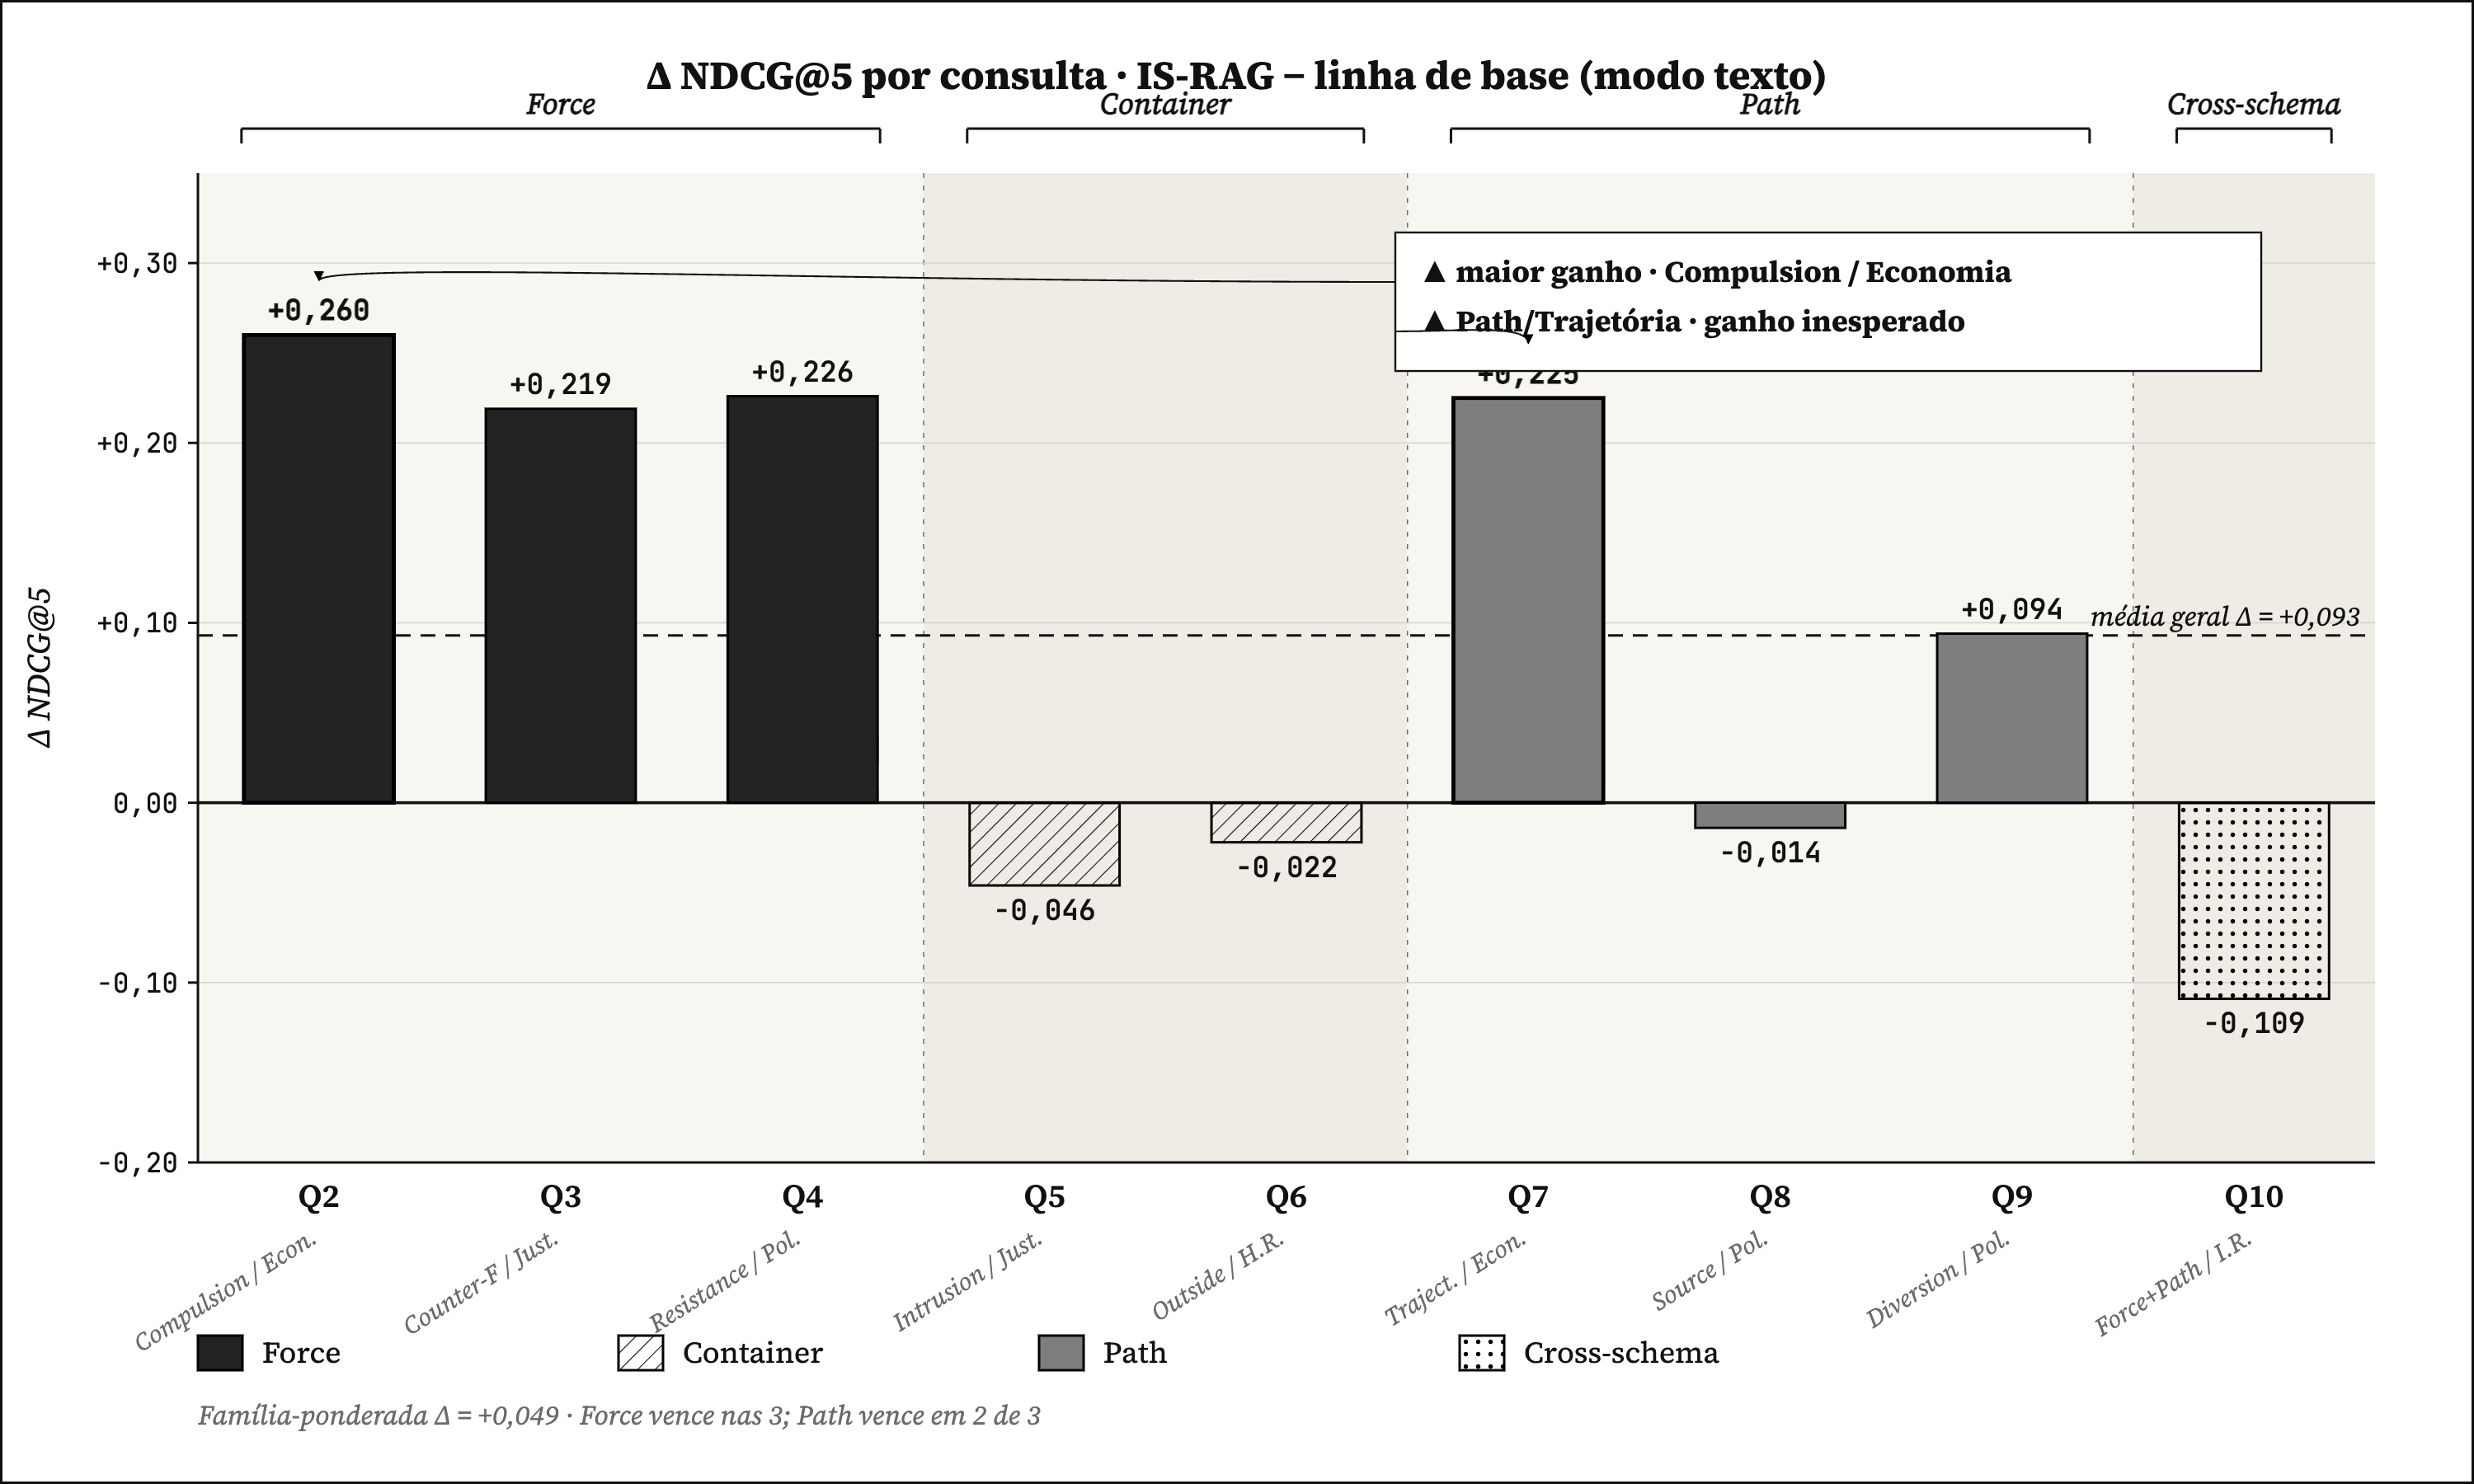
\includegraphics[width=1\textwidth]{images/PT_Results_modo_texto.png}
%  \caption{$\Delta$ NDCG@5 por consulta no modo texto.
%    Resultados completos na Tabela~\ref{tab:perquery};
%    comparação entre modos na Tabela~\ref{tab:modes}.}
%  \label{fig:results}
%\end{figure}

\subsection{Análise por Família de Esquema}

A Tabela~\ref{tab:schema} agrega os resultados do modo texto por
família de esquema (dados completos, 10~consultas).

\begin{table}[H]
\centering
\small
\setlength{\tabcolsep}{4pt}
\begin{tabular}{lccp{4.2cm}}
\toprule
\textbf{Família} & \textbf{$n$} & \textbf{$\Delta$ médio} & \textbf{$\Delta$ individuais} \\
\midrule
\textsc{Force}     & 3 & \textbf{+0,267} & +0,390,\ +0,221,\ +0,189 \\
\textsc{Path}      & 3 & +0,085          & +0,036,\ +0,111,\ +0,109 \\
Cross              & 1 & $-$0,094        & $-$0,094 \\
\textsc{Container} & 3 & $-$0,017        & 0,000,\ $-$0,096,\ +0,046 \\
\midrule
\multicolumn{2}{l}{Média ponderada por família} & +0,060 & \\
\bottomrule
\end{tabular}
\caption{$\Delta$ NDCG@5 por família de esquema (modo texto,
  anotador Opus independente, 10~consultas).
  Famílias ordenadas por $\Delta$ médio. \textsc{Force} é o sinal
  mais forte e consistente; \textsc{Path} é positivo em todas as
  três consultas.}
\label{tab:schema}
\end{table}

\textsc{Force} apresenta o sinal mais forte e consistente
($\Delta = +0{,}267$; todas as três consultas positivas).
\textsc{Path} é positivo em todas as três consultas ($+0{,}085$):
Q8~($+0{,}111$) e Q9~($+0{,}109$) são os maiores ganhos;
Q7~($+0{,}036$) contribui positivamente.
\textsc{Container} apresenta efeito médio próximo de zero ($-0{,}017$),
muito menos severo que nos modos cognitivo e híbrido
(Tabela~\ref{tab:modes_compare}).
Q1, agora avaliável com o anotador Opus, exibe $\Delta{=}0$:
o boost é inerte para o subtipo mais convencionalizado.
A média ponderada por família ($+0{,}060$) confirma que o modo texto
produz resultados positivos na maioria das famílias de esquema.

% =================================================================
\section{Discussão}
\label{sec:discussion}

\paragraph{Force é o maior beneficiário do boosting cognitivo.}
Todas as três consultas \textsc{Force} apresentam $\Delta$ positivo,
com \textsc{Compulsion} ($+$0,390) e \textsc{Counter\_Force}
($+$0,221) como os resultados mais expressivos.
Esquemas \textsc{Force} tendem a empregar vocabulário metafórico
saliente e não convencionalizado no discurso parlamentar
(\emph{pressiona, bloqueia, choca}), tornando a detecção e o boosting
eficazes.
Esse padrão é específico do corpus e não deve ser generalizado sem
validação adicional.

\paragraph{Path é positivo em todas as consultas no modo texto; Container exibe efeito médio próximo de zero.}
No modo híbrido, a consulta \textsc{Path} Q8 degrada severamente
($-0{,}424$), enquanto Q9 é positiva ($+0{,}120$) e Q7 é neutra
($-0{,}007$) (Tabela~\ref{tab:modes_compare}).
No modo texto, todas as três consultas são positivas:
Q8~($+0{,}111$), Q9~($+0{,}109$) e Q7~($+0{,}036$);
a média da família é $+0{,}085$ (Tabela~\ref{tab:schema}).
O déficit pontual de \textsc{Path} no modo híbrido (Q8) é, portanto,
artefato do ruído do embedding cognitivo contaminando a similaridade
base, não uma propriedade intrínseca das metáforas de trajetória.
\textsc{Container} apresenta efeito médio próximo de zero no modo texto
($0{,}000$, $-0{,}096$, $+0{,}046$; média da família $-0{,}017$),
substancialmente menos severo do que no modo híbrido ($-0{,}169$) ou
cognitivo ($-0{,}263$).
\textsc{Container}/\textsc{Intrusion} (Q5) apresenta déficit leve no
modo texto ($-0{,}096$) versus déficit moderado no modo híbrido
($-0{,}191$), ilustrando o padrão geral.

\paragraph{A formulação assertiva das consultas é obrigatória.}
O Analisador Cognitivo aplica uma regra de literalidade: consultas
interrogativas ou analíticas (\emph{``Quais deputados argumentam
que\ldots''}) são corretamente classificadas como não-metafóricas,
retornando listas de esquemas vazias e zerando o boost.
As consultas devem ser formuladas como \emph{afirmações metafóricas
assertivas} para ativar o componente cognitivo.
Esta é uma restrição operacional vinculante para qualquer implantação
do IS-RAG.

\paragraph{Frequência de esquema $\neq$ boostabilidade.}
Q1 foi projetada como \textsc{Container}/\textsc{Inside}, o subtipo
mais frequente no corpus (80~ocorrências).
Com o anotador Haiku, Q1 era excluída (IDCG${=}0$): o modelo atribuía
pontuação~1 a todos os trechos \textsc{Inside} (domínio presente,
esquema não-saliente).
Com o anotador Opus independente, Q1 passa a ter IDCG${>}0$ —
documentos relevantes são identificáveis —, mas o boost IS-RAG
produz $\Delta{=}0$: o esquema é presente mas não discriminativo.
A contenção espacial está tão convencionalizada no discurso parlamentar
que não carrega sinal discriminativo de re-ranking, independentemente
do modelo de julgamento de relevância.
A distribuição final é 3-3-3-1 (10~consultas).

\paragraph{IS-RAG como camada compensatória para limitações de embedding.}
O experimento de embedding (\S\ref{sec:embedding}) posiciona o IS-RAG
dentro de uma tensão arquitetural mais ampla: a lacuna léxico-cognitiva
que o boost de esquemas preenche é justamente aquela que modelos densos
SOTA fecham \emph{implicitamente} por meio de pré-treinamento mais
profundo em corpora multilíngues diversos.
Isso torna o IS-RAG particularmente valioso em cenários de implantação
onde embeddings de grande escala são impraticáveis --- ambientes com
restrição de recursos computacionais, recuperação em dispositivo, ou
contextos regulatórios que exigem modelos hospedados localmente ---
onde o boosting explícito por esquemas recupera parte substancial do
alinhamento semântico que embeddings mais fortes forneceriam nativamente.
À medida que a tecnologia de embedding avança, o valor marginal do
IS-RAG no modo texto tende a diminuir ainda mais, motivando trabalhos
futuros em recuperação ciente de esquemas robusta a embeddings fortes:
ajuste fino específico ao domínio do Analisador Cognitivo,
re-ranqueadores condicionados a esquemas, ou restrições rígidas de
esquema em vez de boosts proporcionais suaves.
Crucialmente, a degradação dos modos híbrido e cognitivo permanece
estável independentemente da qualidade do embedding (\S\ref{sec:embedding}),
confirmando que a falha da recuperação por embedding duplo é estrutural,
não dependente do modelo.

\paragraph{Limitações.}
(1)~O corpus é pequeno e homogêneo (171~trechos, único registro,
somente português); os resultados carecem de testes de significância
estatística.
(2)~\emph{Circularidade com LLM}: o Analisador Cognitivo e o parser
de consulta usam \texttt{claude-haiku-4-5}; o anotador de relevância
usa \texttt{claude-opus-4-7} (configurável via \texttt{ANNOTATOR\_MODEL}).
Essa separação deliberada de modelos rompe o loop de eco mais crítico:
o avaliador não é mais o mesmo modelo que indexou os esquemas dos
documentos.
Risco residual permanece (ambos são modelos Anthropic/Claude), e uma
auditoria humana cega sobre 20\% do pool será conduzida em trabalhos
futuros para calcular o Kappa de Fleiss.
(3)~Confundimento por domínio: as consultas \textsc{Force} se
concentram em Economia e Justiça; se o esquema co-ocorre com esses
domínios no corpus, os ganhos podem refletir afinidade de domínio em
vez de estrutura puramente cognitiva.
(4)~Os pesos de boosting ($\alpha{=}0{,}4$, $\beta{=}0{,}3$) são
escolhas de projeto, não otimizadas.
(5)~\emph{Não-determinismo na avaliação}: o Analisador Cognitivo
introduz variância entre execuções nos scores do IS-RAG.
Uma segunda execução independente produz IS-RAG\,=\,0{,}7716
($\Delta=+0{,}077$, modo texto); a baseline (0{,}6947) é determinística
e estável entre execuções.
A direção positiva de $\Delta$ é consistente entre ambas as execuções;
a magnitude exata não é.
Execuções múltiplas com reporte de média\,$\pm$\,desvio padrão são
deixadas para trabalhos futuros.

% =================================================================
\section{Conclusão}
\label{sec:conclusion}

Este artigo apresenta o IS-RAG como um estudo piloto pioneiro que abre
uma nova linha de pesquisa na interseção entre linguística cognitiva e
recuperação de informação.
A contribuição central não é uma afirmação de superioridade universal,
mas a demonstração de que metadados de esquemas imagéticos podem ser
codificados, detectados e aproveitados como sinal proporcional de
re-ranqueamento dentro de um pipeline de recuperação densa padrão —
produzindo ganho médio de NDCG@5 de $+0{,}091$ no modo texto
(10~consultas, corpus parlamentar brasileiro real).
Uma ablação por modos de recuperação (\S\ref{sec:ablation}) localiza
a contribuição do IS-RAG com precisão: o boost multiplicativo aplicado
sobre a similaridade textual é eficaz
($\Delta_\text{texto} = +0{,}091$), enquanto embeddings cognitivos
usados como vetores de busca degradam o desempenho
($\Delta_\text{híbrido} = -0{,}090$;
$\Delta_\text{cognitivo} = -0{,}192$).
Crucialmente, o ganho no modo texto persiste com anotador independente
(\texttt{claude-opus-4-7} vs.\ \texttt{claude-haiku-4-5}),
descartando eco do LLM como explicação principal
(Tabela~\ref{tab:annotator}).
Um experimento subsequente com \texttt{BAAI/bge-m3}
(\S\ref{sec:embedding}) revela que o ganho é dependente do embedding:
com um modelo multilíngue de última geração, o $\Delta$ no modo texto
colapsa para $\approx 0$, definindo uma fronteira de utilidade para o
boosting cognitivo explícito.

Os resultados assimétricos entre famílias de esquema e modos são em si
achados: revelam que a frequência de um esquema não prediz sua
boostabilidade, que os déficits de \textsc{Path} no modo híbrido são
artefatos de embeddings cognitivos ruidosos — não propriedades do
esquema —, e que a recuperação dual não é necessária para o IS-RAG
funcionar.
O IS-RAG estabelece a prova de conceito e o arcabouço metodológico —
indexação de metadados cognitivos, boosting proporcional, avaliação
estratificada por esquema estilo TREC — sobre os quais trabalhos futuros
em \emph{RI cognitiva} poderão se construir.

Os próximos passos imediatos incluem um design de avaliação cruzada
esquema$\times$domínio, investigação de esquemas convencionalizados
na anotação de relevância graduada, validação em outros registros e
idiomas, e a auditoria humana com Kappa de Fleiss descrita acima.
Convidamos as comunidades de RI e linguística cognitiva a estender,
questionar e refinar esta técnica em corpora mais ricos e arquiteturas
de recuperação mais diversas.

% =================================================================
\paragraph*{Disponibilidade de Código e Dados.}
Código-fonte, corpus e ground truth anotado estão publicamente
disponíveis em \url{https://github.com/yanjustino/is-rag}.

% =================================================================
\bibliography{references}

% =================================================================
\appendix
\setcounter{section}{0}
\renewcommand{\thesection}{\Alph{section}}

% =================================================================
\pagebreak
\section{Algoritmos IS-RAG}
\label{app:algorithms}

\subsection{Pipeline de Indexação}

\begin{algorithm}[H]
\caption{Indexação IS-RAG}\label{alg:index}
\begin{algorithmic}[1]
\Require Corpus $\mathcal{D}$, tamanho de trecho $w{=}150$,
         encoder $\mathcal{E}$, analisador LLM $\mathcal{P}$
\Ensure  Repositório vetorial $\mathcal{S}$ populado
\For{cada documento $d \in \mathcal{D}$}
  \State $C \gets \textsc{SemanticChunk}(d,\,w)$
  \Comment{divisão em fronteiras de sentença}
  \State $\mathbf{E}_t \gets [\,\mathcal{E}(c) \mid c \in C\,]$
  \Comment{embeddings textuais, $d$-dimensional (modelo configurável)}
  \State $M \gets [\,\mathcal{P}(c) \mid c \in C\,]$
  \Comment{chamadas LLM concorrentes, 5 workers}
  \For{$i \gets 1$ \textbf{até} $|C|$}
    \State $\mathbf{e}_c \gets \mathcal{E}(\textsc{Serialize}(M_i))$
    \Comment{embedding cognitivo}
    \State $\mathcal{S}.\textsc{Insert}(C_i,\,\mathbf{E}_{t,i},\,\mathbf{e}_c,\,M_i)$
  \EndFor
\EndFor
\end{algorithmic}
\end{algorithm}

\subsection{Recuperação em Tempo de Consulta}

\begin{algorithm}[H]
\caption{Recuperação IS-RAG}\label{alg:retrieve}
\begin{algorithmic}[1]
\Require Consulta $q$, modo $m \in \{\text{texto, cognitivo, híbrido}\}$,
         top-$k$, repositório $\mathcal{S}$, $\alpha{=}0{,}4$, $\beta{=}0{,}3$
\Ensure  Lista ranqueada de $k$ trechos
\State $(\Sigma_q, \Delta_q) \gets \mathcal{P}(q)$
\Comment{esquemas e domínios detectados}
\State $\mathbf{e}_{q,t} \gets \mathcal{E}(q)$;\;
       $\mathbf{e}_{q,c} \gets \mathcal{E}(\textsc{Serialize}(\mathcal{P}(q)))$
\For{cada trecho $(C_i,\,\mathbf{e}_{t,i},\,\mathbf{e}_{c,i},\,M_i) \in \mathcal{S}$}
  \State $s_t \gets \cos(\mathbf{e}_{q,t},\,\mathbf{e}_{t,i})$;\;
         $s_c \gets \cos(\mathbf{e}_{q,c},\,\mathbf{e}_{c,i})$
  \State $s \gets \begin{cases}
    s_t & \text{se } m = \text{texto} \\
    s_c & \text{se } m = \text{cognitivo} \\
    (s_t + s_c)/2 & \text{se } m = \text{híbrido}
  \end{cases}$
  \State $n \gets |M_i.\text{details}|$
  \State $\sigma \gets |\{d \in M_i.\text{details} \mid d.\text{schema} \in \Sigma_q\}|
                       \;/\; \max(n,1)$
  \State $\delta \gets |\{d \in M_i.\text{details} \mid d.\text{domain} \in \Delta_q\}|
                       \;/\; \max(n,1)$
  \If{$M_i.\text{schemas} \cap \Sigma_q \neq \emptyset$}
    \State $\hat{s}_i \gets s \cdot (1 + \alpha\,\sigma + \beta\,\delta)$
    \Comment{Eq.~\ref{eq:boosting}}
  \Else
    \State $\hat{s}_i \gets s$
    \Comment{sem correspondência de esquema — sem boost}
  \EndIf
\EndFor
\State \Return $\textsc{TopK}(\{\hat{s}_i\},\,k)$
\end{algorithmic}
\end{algorithm}

\end{document}
